\documentclass[a4paper,12pt]{article}

\usepackage[utf8x]{inputenc}
\usepackage[T2A]{fontenc}
\usepackage[english, russian]{babel}

% Опционно, требует  apt-get install scalable-cyrfonts.*
% и удаления одной строчки в cyrtimes.sty
% Сточку не удалять!
% \usepackage{cyrtimes}

% Картнки и tikz
\usepackage{graphicx}
\usepackage{tikz}
\usetikzlibrary{snakes,arrows,shapes}


% Некоторая русификация.
\usepackage{misccorr}
\usepackage{indentfirst}
\renewcommand{\labelitemi}{\normalfont\bfseries{--}}

% Увы, поля придётся уменьшить из-за листингов.
\topmargin -1cm
\oddsidemargin -0.5cm
\evensidemargin -0.5cm
\textwidth 17cm
\textheight 24cm

\sloppy

% Оглавление в PDF
\usepackage[
bookmarks=true,
colorlinks=true, linkcolor=black, anchorcolor=black, citecolor=black, menucolor=black,filecolor=black, urlcolor=black,
unicode=true
]{hyperref}

% Для исходного кода в тексте
\newcommand{\Code}[1]{\texttt{#1}}

\usepackage{verbatim}
\usepackage{fancyvrb}
\fvset{frame=leftline, fontsize=\small, framerule=0.4mm, rulecolor=\color{darkgray}, commandchars=\\\{\}}
\renewcommand{\theFancyVerbLine}{\small\arabic{FancyVerbLine}}


\title{Отчёт по лабораторной работе \\ <<Динамическая IP-маршрутизация>>}
\author{Пучнина Анастасия Ивановна}

\begin{document}

\maketitle

\tableofcontents

\section{Настройка сети}

\subsection{Топология сети}

Топология сети и используемые IP-адреса показаны на рисунке~\ref{fig:network}.

\begin{figure}
\centering
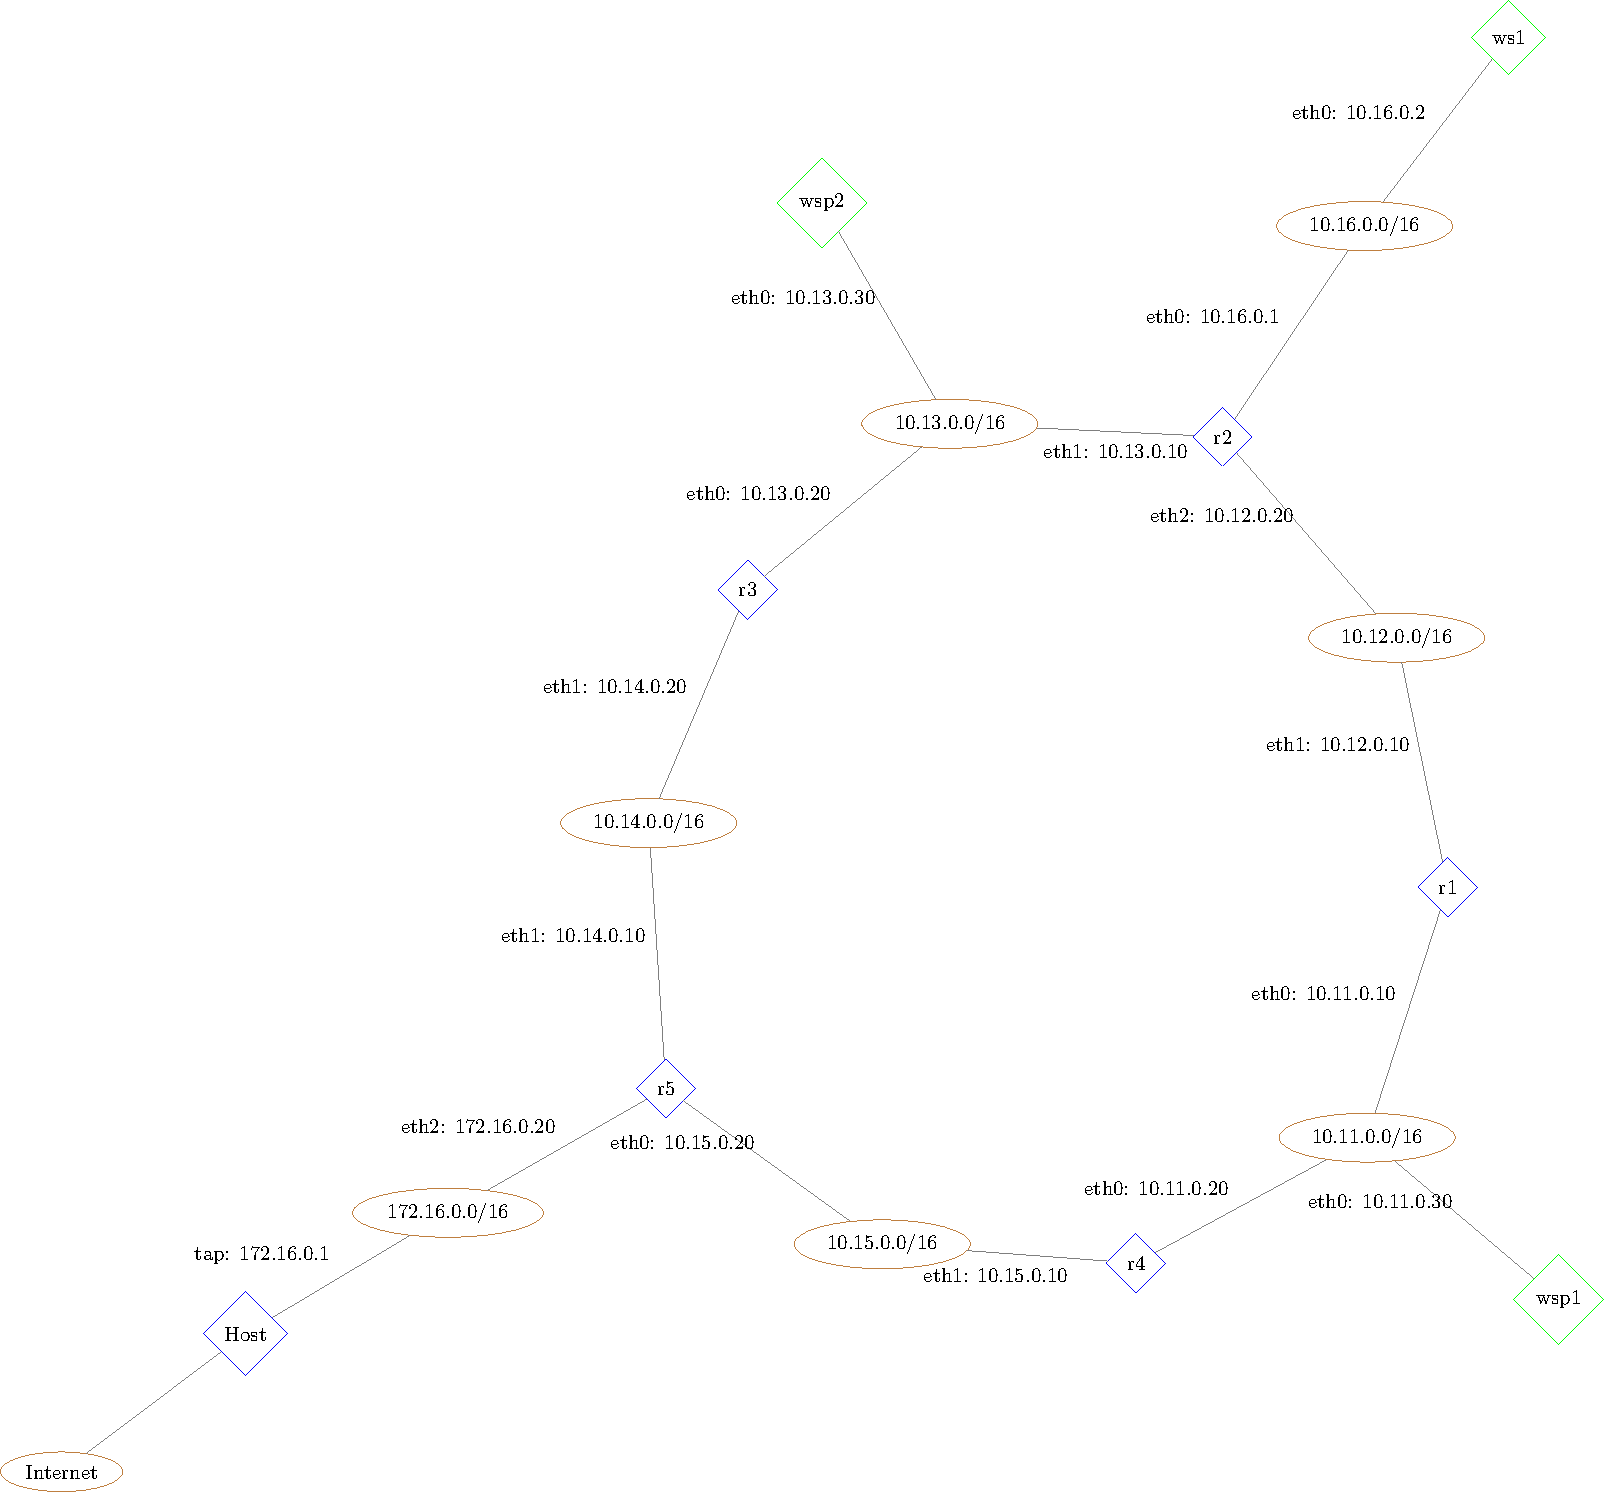
\includegraphics[width=0.8\textwidth]{includes/network_gv.pdf}
\caption{Топология сети}
\label{fig:network}
\end{figure}

Перечень узлов, на которых используется динамическая IP-маршрутизация: r1, r2, r3, r4, r5, wsp1, wsp2


\subsection{Назначение IP-адресов}

Ниже приведён файл сетевой настройки  маршрутизатора (r1).

\begin{Verbatim}
auto lo
iface lo inet loopback

auto eth0
iface eth0 inet static
address 10.11.0.10
netmask 255.255.0.0

auto eth1
iface eth1 inet static
address 10.12.0.10
netmask 255.255.0.0
\end{Verbatim}

Ниже приведён файл сетевой настройки рабочей станции (ws1).

\begin{Verbatim}
auto lo
iface lo inet loopback

auto eth0
iface eth0 inet static
address 10.16.0.2
netmask 255.255.0.0
gateway 10.16.0.1
\end{Verbatim}



\subsection{Настройка протокола RIP}

Ниже приведен файл \Code{/etc/quagga/ripd.conf} маршрутизатора (r5).

\begin{Verbatim}
! Этот настройки, касающиеся протокола RIP.
router rip

! Раскомментируйте ниже все интерфейсы, подключённые
! к сетям с другими маршрутизаторами.
network eth0
network eth1
! network eth2

! Уменьшаем значения всех таймеров для ускорения опытов.
! Рассылка: 10 сек., устаревание: 60 cек., сборка мусора: 120 сек.
timers basic 10 60 120

! Следующие две строчки заставляют маршрутизатор
! добавлять в сообщения протокола RIP все известные ему маршруты.
redistribute kernel
! redistribute connected

! Это имя файла журнала службы RIP.
! Его содержимое можно изучить в случае неполадок
log file /var/log/quagga/ripd.log
\end{Verbatim}


Ниже приведен файл \Code{/etc/quagga/ripd.conf} рабочий станции, связанной с несколькими маршрутизаторами (wsp1).

\begin{Verbatim}
! Этот настройки, касающиеся протокола RIP.
router rip

! Раскомментируйте ниже все интерфейсы, подключённые
! к сетям с другими маршрутизаторами.
network eth0
! network eth1
! network eth2

! Уменьшаем значения всех таймеров для ускорения опытов.
! Рассылка: 10 сек., устаревание: 60 cек., сборка мусора: 120 сек.
timers basic 10 60 120

! Следующие две строчки заставляют маршрутизатор
! добавлять в сообщения протокола RIP все известные ему маршруты.
redistribute kernel
redistribute connected

! Это имя файла журнала службы RIP.
! Его содержимое можно изучить в случае неполадок
log file /var/log/quagga/ripd.log
\end{Verbatim}


\section{Проверка настройки протокола RIP}

Вывод \textbf{traceroute} от узла wsp1 до wsp2 при нормальной работе сети.

\begin{Verbatim}
wsp1:~# traceroute -n 10.13.0.30
traceroute to 10.13.0.30 (10.13.0.30), 64 hops max, 40 byte packets
 1  10.11.0.10  1 ms  0 ms  0 ms
 2  10.12.0.20  2 ms  0 ms  0 ms
 3  10.13.0.30  15 ms  0 ms  0 ms
\end{Verbatim}

Вывод \textbf{traceroute} от узла ws1 до внешнего IP.

\begin{Verbatim}
ws1:~# traceroute -n 188.166.161.195
traceroute to 188.166.161.195 (188.166.161.195), 64 hops max, 40 byte packets
 1  10.16.0.1  0 ms  0 ms  0 ms
 2  10.13.0.20  8 ms  0 ms  0 ms
 3  10.14.0.10  15 ms  0 ms  0 ms
 4  172.16.0.1  1 ms  1 ms  1 ms
 5  * * *
\end{Verbatim}

Вывод сообщения RIP.

\begin{Verbatim}
r1:~#  tcpdump -tnv -i eth0 -s 1518 udp
tcpdump: listening on eth0, link-type EN10MB (Ethernet), capture size 1518 bytes
IP (tos 0x0, ttl 1, id 0, offset 0, flags [DF], proto UDP (17), length 112) 10.11.0.20.520 > 224.0.0.9.520: 
	RIPv2, Response, length: 84, routes: 4
	  AFI: IPv4:         0.0.0.0/0 , tag 0x0000, metric: 2, next-hop: self
	  AFI: IPv4:       10.13.0.0/16, tag 0x0000, metric: 3, next-hop: self
	  AFI: IPv4:       10.14.0.0/16, tag 0x0000, metric: 2, next-hop: self
	  AFI: IPv4:       10.15.0.0/16, tag 0x0000, metric: 1, next-hop: self
\end{Verbatim}

Вывод таблицы RIP.

\begin{Verbatim}
r1# show ip rip
Codes: R - RIP, C - connected, S - Static, O - OSPF, B - BGP
Sub-codes:
      (n) - normal, (s) - static, (d) - default, (r) - redistribute,
      (i) - interface

     Network            Next Hop         Metric From            Tag Time
R(n) 0.0.0.0/0          10.11.0.20            3 10.11.0.20        0 00:54
C(i) 10.11.0.0/16       0.0.0.0               1 self              0
C(i) 10.12.0.0/16       0.0.0.0               1 self              0
R(n) 10.13.0.0/16       10.12.0.20            2 10.12.0.20        0 00:56
R(n) 10.14.0.0/16       10.11.0.20            3 10.11.0.20        0 00:54
R(n) 10.15.0.0/16       10.11.0.20            2 10.11.0.20        0 00:54
R(n) 10.16.0.0/16       10.12.0.20            2 10.12.0.20        0 00:56
\end{Verbatim}

Вывод таблицы маршрутизации.

\begin{Verbatim}
r1:~# ip r
10.16.0.0/16 via 10.12.0.20 dev eth1  proto zebra  metric 2 
10.11.0.0/16 dev eth0  proto kernel  scope link  src 10.11.0.10 
10.14.0.0/16 via 10.11.0.20 dev eth0  proto zebra  metric 3 
10.15.0.0/16 via 10.11.0.20 dev eth0  proto zebra  metric 2 
10.12.0.0/16 dev eth1  proto kernel  scope link  src 10.12.0.10 
10.13.0.0/16 via 10.12.0.20 dev eth1  proto zebra  metric 2 
default via 10.11.0.20 dev eth0  proto zebra  metric 3
\end{Verbatim}

\section{Расщепленный горизонт и испорченные обратные обновления}

Вывод RIPv2 сообщения маршрутизатора r3 с включенным расщепленным горизонтом.

\begin{Verbatim}
tcpdump: listening on eth0, link-type EN10MB (Ethernet), capture size 1518 bytes
IP (tos 0x0, ttl 1, id 0, offset 0, flags [DF], proto UDP (17), length 112) 10.13.0.20.520 > 224.0.0.9.520: 
	RIPv2, Response, length: 84, routes: 4
	  AFI: IPv4:         0.0.0.0/0 , tag 0x0000, metric: 2, next-hop: self
	  AFI: IPv4:       10.11.0.0/16, tag 0x0000, metric: 3, next-hop: self
	  AFI: IPv4:       10.14.0.0/16, tag 0x0000, metric: 1, next-hop: self
	  AFI: IPv4:       10.15.0.0/16, tag 0x0000, metric: 2, next-hop: self
\end{Verbatim}

Как мы видим, при рассылке с учётом правила расщепленного горизонта, данные таблицы RIP для подсетей 10.13.0.0/16, 10.12.0.0/16, 10.16.0.0/16 не отправляются с интерфейса eth0, так как информация об этих маршрутах была получена с данного интерфейса. 


Вывод RIPv2 сообщения маршрутизатора r3 с включенным испорченными обновлениями.

\begin{Verbatim}
IP (tos 0x0, ttl 1, id 0, offset 0, flags [DF], proto UDP (17), length 172) 10.13.0.20.520 > 224.0.0.9.520: 
	RIPv2, Response, length: 144, routes: 7
	  AFI: IPv4:         0.0.0.0/0 , tag 0x0000, metric: 2, next-hop: self
	  AFI: IPv4:       10.11.0.0/16, tag 0x0000, metric: 3, next-hop: self
	  AFI: IPv4:       10.12.0.0/16, tag 0x0000, metric: 16, next-hop: 10.13.0.10
	  AFI: IPv4:       10.13.0.0/16, tag 0x0000, metric: 16, next-hop: self
	  AFI: IPv4:       10.14.0.0/16, tag 0x0000, metric: 1, next-hop: self
	  AFI: IPv4:       10.15.0.0/16, tag 0x0000, metric: 2, next-hop: self
	  AFI: IPv4:       10.16.0.0/16, tag 0x0000, metric: 16, next-hop: 10.13.0.10
\end{Verbatim}

При использовании правила испорченного обратно обновления, информация о таких маршрутах включается в сообщение, но метрика таких маршрутов равна 16 (бесконечности).


Вывод RIPv2 сообщения маршрутизатора r3 с отключенным расщепленным горизонтом.

\begin{Verbatim}
IP (tos 0x0, ttl 1, id 0, offset 0, flags [DF], proto UDP (17), length 172) 10.13.0.20.520 > 224.0.0.9.520: 
	RIPv2, Response, length: 144, routes: 7
	  AFI: IPv4:         0.0.0.0/0 , tag 0x0000, metric: 2, next-hop: self
	  AFI: IPv4:       10.11.0.0/16, tag 0x0000, metric: 3, next-hop: 10.13.0.10
	  AFI: IPv4:       10.12.0.0/16, tag 0x0000, metric: 2, next-hop: 10.13.0.10
	  AFI: IPv4:       10.13.0.0/16, tag 0x0000, metric: 1, next-hop: self
	  AFI: IPv4:       10.14.0.0/16, tag 0x0000, metric: 1, next-hop: self
	  AFI: IPv4:       10.15.0.0/16, tag 0x0000, metric: 2, next-hop: self
	  AFI: IPv4:       10.16.0.0/16, tag 0x0000, metric: 2, next-hop: 10.13.0.10
\end{Verbatim}

При отключении правила, метрика описанных выше маршрутов устанавливается в реальное значение, хранимое в таблице RIP, однако учитываться маршрутизатором-получателем данные метрики будут навряд ли, так как значение новой полученной метрики из сообщения должно быть больше на единицу, чем у получателя.

Вернём настройки в исходное состояние (включенный без испорченных).

\section{Имитация устранимой поломки в сети}

Вывод \textbf{traceroute} от узла такого-то до такого-то после того, как служба RIP перестроила таблицы маршрутизации.

\begin{Verbatim}
ws1:~# traceroute -n 10.11.0.30
traceroute to 10.11.0.30 (10.11.0.30), 64 hops max, 40 byte packets
 1  10.16.0.1  0 ms  0 ms  0 ms
 2  10.12.0.10  11 ms  0 ms  0 ms
 3  10.11.0.30  10 ms  0 ms  0 ms
\end{Verbatim}

Отключим маршрутизатор r1 для наблюдения за поведением маршрутизаторов при устранимой поломке в сети.

Вывод таблицы RIP непосредственно перед истечением таймера устаревания (на маршрутизаторе-соседе отключенного).

\begin{Verbatim}
r4# show ip rip
Codes: R - RIP, C - connected, S - Static, O - OSPF, B - BGP
Sub-codes:
      (n) - normal, (s) - static, (d) - default, (r) - redistribute,
      (i) - interface

     Network            Next Hop         Metric From            Tag Time
R(n) 0.0.0.0/0          10.15.0.20            2 10.15.0.20        0 00:55
C(i) 10.11.0.0/16       0.0.0.0               1 self              0
R(n) 10.12.0.0/16       10.11.0.10            2 10.11.0.10        0 00:12
R(n) 10.13.0.0/16       10.11.0.10            3 10.11.0.10        0 00:12
R(n) 10.14.0.0/16       10.15.0.20            2 10.15.0.20        0 00:55
C(i) 10.15.0.0/16       0.0.0.0               1 self              0
R(n) 10.16.0.0/16       10.11.0.10            3 10.11.0.10        0 00:12
\end{Verbatim}

Перестроенная таблица на этом же маршрутизаторе

\begin{Verbatim}
r4# show ip rip
Codes: R - RIP, C - connected, S - Static, O - OSPF, B - BGP
Sub-codes:
      (n) - normal, (s) - static, (d) - default, (r) - redistribute,
      (i) - interface

     Network            Next Hop         Metric From            Tag Time
R(n) 0.0.0.0/0          10.15.0.20            2 10.15.0.20        0 00:57
C(i) 10.11.0.0/16       0.0.0.0               1 self              0
R(n) 10.12.0.0/16       10.11.0.10           16 10.11.0.10        0 01:55
R(n) 10.13.0.0/16       10.15.0.20            3 10.15.0.20        0 00:57
R(n) 10.14.0.0/16       10.15.0.20            2 10.15.0.20        0 00:57
C(i) 10.15.0.0/16       0.0.0.0               1 self              0
R(n) 10.16.0.0/16       10.15.0.20            4 10.15.0.20        0 00:57
\end{Verbatim}


Вывод \textbf{traceroute} от узла такого-то до такого-то после того, как служба RIP перестроила таблицы маршрутизации.

\begin{Verbatim}
ws1:~# traceroute -n 10.11.0.30
traceroute to 10.11.0.30 (10.11.0.30), 64 hops max, 40 byte packets
 1  10.16.0.1  1 ms  1 ms  0 ms
 2  10.13.0.20  11 ms  0 ms  0 ms
 3  10.14.0.10  11 ms  1 ms  0 ms
 4  10.15.0.10  6 ms  0 ms  0 ms
 5  10.11.0.30  11 ms  0 ms  0 ms
\end{Verbatim}

\section{Имитация неустранимой поломки в сети}

Отключим маршрутизатор r3, чтобы сеть перестала быть связанной.
Ниже приведены таблицы маршрутизации RIP маршрутизатора r5 после отключения маршрутизатора r3.

\begin{Verbatim}
r5# show ip rip
Codes: R - RIP, C - connected, S - Static, O - OSPF, B - BGP
Sub-codes:
      (n) - normal, (s) - static, (d) - default, (r) - redistribute,
      (i) - interface

     Network            Next Hop         Metric From            Tag Time
K(r) 0.0.0.0/0          172.16.0.1            1 self              0
R(n) 10.11.0.0/16       10.15.0.10            2 10.15.0.10        0 00:57
R(n) 10.12.0.0/16       10.14.0.20            3 10.14.0.20        0 00:01
R(n) 10.13.0.0/16       10.14.0.20            2 10.14.0.20        0 00:01
C(i) 10.14.0.0/16       0.0.0.0               1 self              0
C(i) 10.15.0.0/16       0.0.0.0               1 self              0
R(n) 10.16.0.0/16       10.14.0.20            3 10.14.0.20        0 00:01
r5# show ip rip
Codes: R - RIP, C - connected, S - Static, O - OSPF, B - BGP
Sub-codes:
      (n) - normal, (s) - static, (d) - default, (r) - redistribute,
      (i) - interface

     Network            Next Hop         Metric From            Tag Time
K(r) 0.0.0.0/0          172.16.0.1            1 self              0
R(n) 10.11.0.0/16       10.15.0.10            2 10.15.0.10        0 00:54
R(n) 10.12.0.0/16       10.14.0.20           16 10.14.0.20        0 01:58
R(n) 10.13.0.0/16       10.14.0.20           16 10.14.0.20        0 01:58
C(i) 10.14.0.0/16       0.0.0.0               1 self              0
C(i) 10.15.0.0/16       0.0.0.0               1 self              0
R(n) 10.16.0.0/16       10.14.0.20           16 10.14.0.20        0 01:58
\end{Verbatim}

Отправка маршрутизатором r5 сообщений RIP с метрикой 16.

\begin{Verbatim}
r5:~# tcpdump -tnv -i eth0 -s 1518 udp
tcpdump: listening on eth0, link-type EN10MB (Ethernet), capture size 1518 bytes
IP (tos 0x0, ttl 1, id 0, offset 0, flags [DF], proto UDP (17), length 132) 10.15.0.20.520 > 224.0.0.9.520: 
	RIPv2, Response, length: 104, routes: 5
	  AFI: IPv4:         0.0.0.0/0 , tag 0x0000, metric: 1, next-hop: self
	  AFI: IPv4:       10.12.0.0/16, tag 0x0000, metric: 16, next-hop: self
	  AFI: IPv4:       10.13.0.0/16, tag 0x0000, metric: 16, next-hop: self
	  AFI: IPv4:       10.14.0.0/16, tag 0x0000, metric: 1, next-hop: self
	  AFI: IPv4:       10.16.0.0/16, tag 0x0000, metric: 16, next-hop: self
\end{Verbatim}

\end{document}
